%\documentclass[aspectratio=169]{beamer}
\documentclass[aspectratio=43]{beamer}
% \usepackage[utf8]{inputenc}
\usepackage{multicol}
\usepackage[bigfiles]{pdfbase}

% \AtBeginSection[]
% {
%     \begin{frame}
%         \frametitle{Table of Contents}
%         \tableofcontents[currentsection]
%     \end{frame}
% }


%% Useful packages
\usepackage{amsmath}
\usepackage{graphicx}
\graphicspath{{fig/}}
\usepackage{xcolor}
\usepackage{tikz}
% \usepackage[hidelinks]{hyperref}

\newcommand{\height}{H}
\newcommand{\av}[1]{\langle {#1} \rangle}
\newcommand{\vect}[1]{\mathbf{#1}}

\newlength{\wdth}
\newcommand{\strike}[1]{\settowidth{\wdth}{#1}\rlap{\rule[.5ex]{\wdth}{.4pt}}#1}


% \title{3D-PTV with FPGA for Lagrangian measurements in a wind tunnel}
\title{Towards a real-time three-dimensional particle tracking velocimetry (3D-PTV)}
% \date{July 9, 2018}
\date{June 19-21, 2023}
\author[Liberzon]{Alex Liberzon, Tel Aviv University}


\usetheme{material}

\useDarkTheme
%\useLightTheme
%\usePrimaryRed
\usePrimaryPink
%\usePrimaryBlueGrey
%\useAccentGreen
\useAccentPurple
%\useAccentWhite
%\useAccentIndigo

\usepackage[sfdefault]{roboto}
\setbeamertemplate{footline}[frame number]
%%%%%%%%%%%%%%%%%%%%%%%%%%%%%%%%%%%%%%%%%%%%%%%%%%%%%%%%%%%%%%%%%%%%%%%%%%%%%%
% \embedvideo{<poster or text>}{<video file (MP4+H264)>}
% \embedvideo*{...}{...}                     % auto-play
%%%%%%%%%%%%%%%%%%%%%%%%%%%%%%%%%%%%%%%%%%%%%%%%%%%%%%%%%%%%%%%%%%%%%%%%%%%%%%

\ExplSyntaxOn
\NewDocumentCommand\embedvideo{smm}{
  \group_begin:
  \leavevmode
  \tl_if_exist:cTF{file_\file_mdfive_hash:n{#3}}{
    \tl_set_eq:Nc\video{file_\file_mdfive_hash:n{#3}}
  }{
    \IfFileExists{#3}{}{\GenericError{}{File~`#3'~not~found}{}{}}
    \pbs_pdfobj:nnn{}{fstream}{{}{#3}}
    \pbs_pdfobj:nnn{}{dict}{
      /Type/Filespec/F~(#3)/UF~(#3)
      /EF~<</F~\pbs_pdflastobj:>>
    }
    \tl_set:Nx\video{\pbs_pdflastobj:}
    \tl_gset_eq:cN{file_\file_mdfive_hash:n{#3}}\video
  }
  %
  \pbs_pdfobj:nnn{}{dict}{
    /Type/RichMediaInstance/Subtype/Video
    /Asset~\video
    /Params~<</FlashVars (
      source=#3&
      skin=SkinOverAllNoFullNoCaption.swf&
      skinAutoHide=true&
      skinBackgroundColor=0x5F5F5F&
      skinBackgroundAlpha=0
    )>>
  }
  %
  \pbs_pdfobj:nnn{}{dict}{
    /Type/RichMediaConfiguration/Subtype/Video
    /Instances~[\pbs_pdflastobj:]
  }
  %
  \pbs_pdfobj:nnn{}{dict}{
    /Type/RichMediaContent
    /Assets~<<
      /Names~[(#3)~\video]
    >>
    /Configurations~[\pbs_pdflastobj:]
  }
  \tl_set:Nx\rmcontent{\pbs_pdflastobj:}
  %
  \pbs_pdfobj:nnn{}{dict}{
    /Activation~<<
      /Condition/\IfBooleanTF{#1}{PV}{XA}
      /Presentation~<</Style/Embedded>>
    >>
    /Deactivation~<</Condition/PI>>
  }
  %
  \hbox_set:Nn\l_tmpa_box{#2}
  \tl_set:Nx\l_box_wd_tl{\dim_use:N\box_wd:N\l_tmpa_box}
  \tl_set:Nx\l_box_ht_tl{\dim_use:N\box_ht:N\l_tmpa_box}
  \tl_set:Nx\l_box_dp_tl{\dim_use:N\box_dp:N\l_tmpa_box}
  \pbs_pdfxform:nnnnn{1}{1}{}{}{\l_tmpa_box}
  %
  \pbs_pdfannot:nnnn{\l_box_wd_tl}{\l_box_ht_tl}{\l_box_dp_tl}{
    /Subtype/RichMedia
    /BS~<</W~0/S/S>>
    /Contents~(embedded~video~file:#3)
    /NM~(rma:#3)
    /AP~<</N~\pbs_pdflastxform:>>
    /RichMediaSettings~\pbs_pdflastobj:
    /RichMediaContent~\rmcontent
  }
  \phantom{#2}
  \group_end:
}
\ExplSyntaxOff

% \includeonlyframes{intro-*}
% \includeonlyframes{ptv-*}
% \includeonlyframes{Intro-*,Sss-Slide2}

\makeatletter
\def\beamer@checkifinlist#1,#2\relax{%
\def\beamer@temp{#1}%
\let\b@name\beamer@againname
\b@star@test#1\relax-*!\relax\count@
\ifx\beamer@temp\b@name
\else
  \def \beamer@temp {#2}%
  \ifx\beamer@temp\@empty
    \gdef\beamer@whichframes{all:0}%
  \else
    \beamer@checkifinlist#2\relax
  \fi
\fi }

\def\b@star@test#1-*#2\relax#3\count@{%
\ifx\\#2\\%
\def\beamer@temp{#1}%
\expandafter\b@dash@test\beamer@againname-\valign\relax
\fi}

\def\b@dash@test#1-#2#3\relax{%
\ifx\valign#2%
\else
\def\b@name{#1}%
\fi}
\makeatother

%%%%%%%%%%%%%%%%%%%%%%%%%%%%%%%%%%%%%%%%
\begin{document}

\begin{frame}
    \titlepage
\end{frame}

\begin{frame}\frametitle{Outline}
    \begin{card}	
    \tableofcontents
    \end{card}
\end{frame}

% \begin{frame}{Hourglass - credit: \href{https://www.youtube.com/shorts/IEtQHRVqI7s}{shortvideos1250 Youtube}}
% \embedvideo{\cardImg[height=.8\textheight]{hourglass}{.9\textwidth}}{video/hourglass.mp4}
% \end{frame}

% \section{Outline}
\section{Introduction}
\topicFramePrimary{Introduction}
%\section{Summary and conclusions}

\begin{frame}
\frametitle{Introduction}
\begin{itemize}
\item Briefly introduce yourself and your background in real-time 3D-PTV.
\item Provide an overview of what real-time 3D-PTV is and why it is important.
\end{itemize}
\end{frame}

% \documentclass{beamer}
% \usepackage{multicol}
% \usepackage{graphicx}
% \graphicspath{{./fig/}}
% \usetheme{material}


% \begin{document}

% \subsection{My path to 3DPTV}
%

\begin{frame}[label=intro-1]{
\includegraphics[width=0.035\textwidth]{qrcode} Alex Liberzon - my trajectory }

\begin{columns}
\begin{column}{.78\textwidth}
\begin{card}
\begin{itemize}
\item Odessa National Polytechnic University, Ukraine
\item Technion - Israel Institute of Technology, Israel
\item ETH Z\"{u}rich, Switzerland
%\item St. Anthony Falls Laboratory, MN, USA
\item Tel Aviv University, Israel
\end{itemize}
\end{card}
\end{column}

    \begin{column}{.02\textwidth}
        \rule{.1mm}{0.7\textheight}
    \end{column}
    
\begin{column}{.2\textwidth}
\cardImg{fig/career/onpu.jpg}{.7\textwidth}
\cardImg{fig/career/technion.png}{.7\textwidth}
\cardImg{fig/career/eth.jpg}{.7\textwidth}
\cardImg{TAU_logo}{.7\textwidth}
% \cardImg{fig/career/lab.jpg}{.25\textwidth}
\end{column}
\end{columns}
\end{frame}
%
\begin{frame}[label=intro-2]
\frametitle{
\includegraphics[width=0.035\textwidth]{github.jpeg} All my work is open sourced  }
\begin{multicols}{2}
\begin{card}
\begin{itemize}
\item OpenPIV
\item OpenPTV
\item PyPTV
\item MothPy
\item SciMED
\item AlgaeFarm
\end{itemize}
\end{card}
\cardImg{openpiv}{.3\textwidth} 
\cardImg{openptv}{.3\textwidth}
\cardImg{pyptv}{.3\textwidth}
\end{multicols}
\end{frame}

\begin{frame}[label=intro-3]{Tel Aviv University \href{http://www.youtube.com/watch?v=rbUevEuYQHg}{ ...  promotional video}}
\begin{multicols}{2}
\centering
\cardImg{telaviv}{.48\textwidth} \cardImg{sculpture_tau_polymer}{0.48\textwidth}
\cardImg{telaviv2}{.48\textwidth}\cardImg{wolfson}{0.48\textwidth}
\end{multicols}
\end{frame}


\begin{frame}[label=intro-4]{International students are welcome - see this opportunity}
\begin{center}
\cardImg{open_week_tau}{.7\textwidth}
\end{center}
\end{frame}

% \end{document}


\begin{frame}
\frametitle{Importance of real-time 3D-PTV}
\begin{itemize}
\item Explain how real-time 3D-PTV provides unique benefits, such as nearly real-time results, that are unavailable through other methods.
\item Describe some of the potential applications of real-time 3D-PTV, such as in fluid dynamics, combustion, and biomedical engineering.
\item Present some examples of successful real-time 3D-PTV projects to illustrate their utility.
\end{itemize}
\end{frame}

\section{Importance of real-time 3D-PTV}
\topicFramePrimary{Why real-time 3D-PTV ? }
\section{Why real-time}


\begin{frame}[label=intro]
\frametitle{We start with a happy end story}
\cardImg{Ron.jpg}{0.8\textwidth}
\begin{cardTiny}
Ron Shnapp is a faculty at the Ben Gurion University, but it could turn out differently. 
\end{cardTiny}
\end{frame}

\begin{frame}{The Conceptual Advantage of Real-Time Information for Measurement Systems}

\begin{itemize}
\item Real-time information gives users a better understanding of the measurement process and enables them to make more informed decisions based on the data.
\item Real-time information allows users to monitor the measurement process in real time and detect any anomalies or issues as they occur.
\item Real-time information about uncertainties allows users better to understand the reliability and accuracy of the measured data.
\item Real-time information about uncertainties can help users optimize the measurement process itself.
\end{itemize}

\end{frame}

\begin{frame}{Real-Time Information Enables Effective Troubleshooting and Maintenance}

\begin{itemize}
\item Real-time information allows for quick and effective troubleshooting and maintenance, which can help prevent further errors or inaccuracies.
\item Early detection of issues is critical in safety-critical systems where even a small delay in detecting a problem can have serious consequences.
\end{itemize}

\end{frame}

\begin{frame}{Real-Time Information Improves Accuracy and Precision}

\begin{itemize}
\item Real-time information allows users to adjust the measurement process in real-time to improve accuracy and precision.
\item Real-time information about uncertainties allows users to make more informed decisions about how to use the data and what level of confidence they can have in the results.
\item Real-time monitoring of uncertainties can help users optimize the measurement process and reduce uncertainties to improve overall accuracy and precision.
\end{itemize}

\end{frame}

\begin{frame}{Real-Time Information Enables Faster Decision-Making}

\begin{itemize}
\item Real-time output allows for faster decision-making by providing immediate feedback on the measured data.
\item Real-time information is especially important in time-sensitive applications where quick decisions can make a significant difference.
\end{itemize}

\end{frame}

\begin{frame}{Real-Time Information Enables Process Control}

\begin{itemize}
\item Real-time output can be used to monitor and control processes in real time, allowing for adjustments to be made as needed to ensure optimal performance.
\item Real-time information is especially important in manufacturing and industrial applications where process control can impact quality, safety, and efficiency.
\end{itemize}

\end{frame}

\begin{frame}{Real-Time Information Enables Remote Monitoring}

\begin{itemize}
\item Real-time output can enable remote monitoring of measurement systems, allowing users to monitor and control systems from a distance.
\item Real-time information is especially important in applications where access to the measurement system may be limited or difficult.
\end{itemize}

\end{frame}

\subsection{Why real-time 3D-PTV}

\begin{frame}{Advantages of Real-Time 3D-PTV}

\begin{itemize}
\item Real-time 3D-PTV allows for immediate feedback on the velocity field, which can be used for process control and optimization.
\item Real-time 3D-PTV enables faster decision-making by providing immediate feedback on the fluid flow behavior, allowing for quick adjustments to be made as needed.
\item Real-time 3D-PTV can provide detailed insight into the fluid flow behavior, which can be used for research purposes and to improve understanding of fluid dynamics.
\item Real-time 3D-PTV can help improve the accuracy and precision of the measured data by allowing for adjustments to be made in real-time to reduce uncertainties.
\item Real-time 3D-PTV can help detect any anomalies or issues in the fluid flow behavior as they occur, allowing for quick and effective troubleshooting and maintenance.
\item Real-time 3D-PTV can be used to remotely monitor fluid flow behavior, which can be especially important in applications where access to the measurement system may be limited or difficult.
\end{itemize}

\end{frame}

\begin{frame}{Immediate Feedback for Process Control and Optimization}

\begin{itemize}
\item Real-time 3D-PTV allows for immediate feedback on the velocity field, which can be used for process control and optimization.
\item Faster decisions can be made to adjust the process as needed, ensuring optimal performance and efficiency.
\end{itemize}

\end{frame}

\begin{frame}{Faster Decision-Making}

\begin{itemize}
\item Real-time 3D-PTV enables faster decision-making by providing immediate feedback on the fluid flow behavior, allowing for quick adjustments to be made as needed.
\item Faster decisions can help prevent delays and improve overall efficiency in applications where time is critical.
\end{itemize}

\end{frame}

\begin{frame}{Detailed Insight into Fluid Dynamics}

\begin{itemize}
\item Real-time 3D-PTV can provide detailed insight into the fluid flow behavior, which can be used for research purposes and to improve understanding of fluid dynamics.
\item More detailed information can lead to new discoveries and improvements in fluid dynamics research.
\end{itemize}

\end{frame}

\begin{frame}{Improved Accuracy and Precision}

\begin{itemize}
\item Real-time 3D-PTV can help improve the accuracy and precision of the measured data by allowing for adjustments to be made in real-time to reduce uncertainties.
\item Real-time monitoring of uncertainties can help reduce errors and improve confidence in the measured data.
\end{itemize}

\end{frame}

\begin{frame}{Effective Troubleshooting and Maintenance}

\begin{itemize}
\item Real-time 3D-PTV can help detect any anomalies or issues in the fluid flow behavior as they occur, allowing for quick and effective troubleshooting and maintenance.
\item Early detection of issues is critical in safety-critical applications where delays can have serious consequences.
\end{itemize}

\end{frame}

\begin{frame}{Remote Monitoring}

\begin{itemize}
\item Real-time 3D-PTV can be used to remotely monitor fluid flow behavior, which can be especially important in applications where access to the measurement system may be limited or difficult.
\item Remote monitoring can allow for more efficient use of resources and improve safety in hazardous environments.
\end{itemize}

\end{frame}

\begin{frame}
\frametitle{Feasibility and Difficulty}
\begin{itemize}
\item Discuss the technical feasibility of real-time 3D-PTV and the challenges that must be overcome to achieve it.
\item Highlight some of the key research areas that need to be addressed to make real-time 3D-PTV more feasible and efficient.
\item Provide examples of some of the tools and resources available to help researchers in this area.
\end{itemize}
\end{frame}


\section{Feasibility and Difficulty}
\topicFramePrimary{Navigating the Path to 3D-PTV: Essential Factors and Prerequisites}
% \documentclass{beamer}
% \usepackage{multicol}
% \usepackage{graphicx}
% \graphicspath{{./fig/}}
% \usetheme{material}


% \begin{document}

\section{3D-PTV Overview}

\begin{frame}[label=ptv-1]{Fluid dynamicists in the audience?}
\centering\cardImg[height]{7j34up.jpg}{.8\textwidth}
\end{frame}


\begin{frame}[label=ptv-21]{3D-PTV overview}
\begin{multicols}{2}
\begin{card}[What is 3D-PTV]
3D-PTV is a technique that allows tracking of particles in three-dimensional space for improved fluid dynamics understanding, using the Lagrangian framework
\end{card}
\begin{card}[How does it work?]
Multiple 2D projections of the particles are obtained and overlapped to create 3D reconstruction. Software than tracks the particles' positions through sequential images over time. 
\end{card}
\end{multicols}
\end{frame}


%
\begin{frame}[label=ptv-211]{Overview from Shr\"{o}der and Schanz, Annu. Rev. Fluid Mech. 2023}
\cardImg{shroder.jpeg}{\textwidth}
\end{frame}

\begin{frame}[label=ptv-3]{What is this Lagrangian framework?}
\centering\cardImg{art}{0.8\textwidth}
\vspace{-.3cm}
\begin{cardTiny}
``Marianthe'' invited people inside turbulent forms to experience them as
if they were a particle borne along in the flow. Athena
Tacha (1985), \href{http://nautil.us/issue/15/turbulence/the-scientific-problem-that-must-be-experienced}{``Nautilus'' by Philip Ball}
\end{cardTiny}
\end{frame}
%

\begin{frame}[label=ptv-4]{Quick intro to 3D-PTV}
\cardImg{ptv-scheme}{1.0\textwidth}
\end{frame}
% % 
% % %
% \begin{frame}[label=ptv-2]{Basic steps}
% \begin{columns}[t]
% 	\begin{column}{0.4\textwidth}
% 		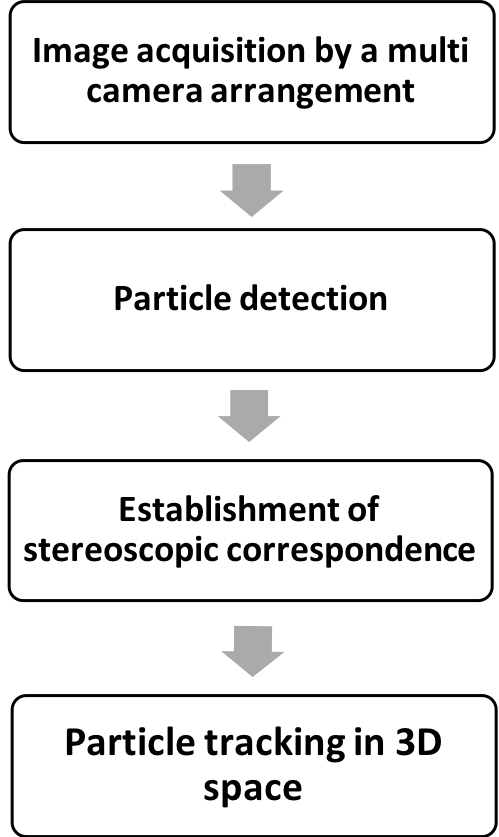
\includegraphics[height=.8\textheight]{ptv_blocks}
% 	\end{column}
% 	\begin{column}{0.3\textwidth}
% 		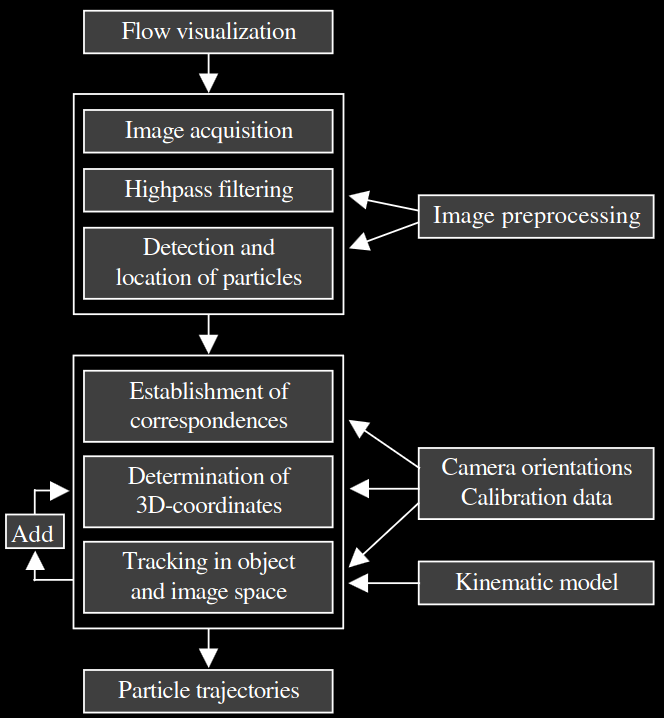
\includegraphics[height=.8\textheight]{ptv_steps}
% 	\end{column}
% \end{columns}
% \end{frame}


\begin{frame}[label=ptv-2]{Basic steps of 3D-PTV}
\centering\cardImg[height=.8\textheight]{ptv_steps}{\textwidth}
\end{frame}

% %%
% \begin{frame}[label=ptv-22]{Basic steps}
% \begin{multicols*}{2}
% 		\cardImg[height]{ptv_blocks}{.49\textwidth}
% 		\cardImg[height]{ptv_steps}{.49\textwidth}
% \end{multicols*}
% \end{frame}

\begin{frame}[label=ptv-5]{Epipolar geometry}
\centering\cardImg{epipolar1}{1\textwidth}
\end{frame}

\begin{frame}[label=ptv-51]{Multi-view epipolar geometry}
\centering\cardImg{epipolar}{\textwidth}
\end{frame}

\begin{frame}[label=ptv-51a]{Multi-view epipolar geometry}
\centering\cardImg{stereo_matching}{\textwidth}
\end{frame}

\begin{frame}[label=ptv-55]{Multi-view epipolar geometry depends on calibration}
\centering\cardImg{calibration1}{\textwidth}
\end{frame}

	

\begin{frame}[label=ptv-6]{Four frames sliding tracking}
\centering\cardImg{tracking}{1\textwidth}
\end{frame}

\begin{frame}[label=ptv-61]{Tracking in 2D space}
\centering\cardImg[height=.8\textheight]{tracking_in_image_space_projection}{1\textwidth}
\end{frame}


\begin{frame}[label=ptv-61a]{Tracking in 2D space}
	\centering\cardImg[height=.8\textheight]{tracking_in_image_space}{1\textwidth}
\end{frame}

\begin{frame}[label=ptv-61b]{Tracking in 3D }
	\centering\cardImg[height=.8\textheight]{tracking_in_3d_space}{1\textwidth}
\end{frame}

\begin{frame}[label=ptv-61c]{Tracking in both 2D and 3D}
	\centering\cardImg[height=.8\textheight]{image_space_tracking}{1\textwidth}
\end{frame}

			

\begin{frame}[label=ptv-7]{The results are Lagrangian trajectories}
\centering
\cardImg{lagrangian_trajectory}{.49\textwidth}
\cardImg{particle_trajectories}{.49\textwidth}
\end{frame}

\begin{frame}[label=ptv-71]{Two frame PTV is Eulerian, not Lagrangian}
\centering\cardImg{eulerian_vs_lagrangian}{\textwidth}
\end{frame}

\begin{frame}[label=ptv-8]
\frametitle{Time-resolved is a tautology, real-time is real :) }
\begin{enumerate}
\item Time-resolved PTV is a tautology - to track objects we have to resolve their position in time :) 
\item Real-time is not at the velocity of the particle, but during the experiment: we get trajectories on the screen when the flow is moving (not the same flow)
\end{enumerate}
\end{frame}

 % \end{document}
\topicFramePrimary{From 3D-PTV towards real-time 3D-PTV}
% \documentclass{beamer}
% \usepackage{graphicx}
% \usepackage{multicol}
% \setlength{\columnseprule}{1pt}

% \graphicspath{{./fig/}}
% \usetheme{material}
% %%%%%%%%%%%%%%%%%%%%%%%%%%%%%%%%%%%%%%%%%%%%%%%%%%%%%%%%%%%%%%%%%%%%%%%%%%%%%%
% \embedvideo{<poster or text>}{<video file (MP4+H264)>}
% \embedvideo*{...}{...}                     % auto-play
%%%%%%%%%%%%%%%%%%%%%%%%%%%%%%%%%%%%%%%%%%%%%%%%%%%%%%%%%%%%%%%%%%%%%%%%%%%%%%

\ExplSyntaxOn
\NewDocumentCommand\embedvideo{smm}{
  \group_begin:
  \leavevmode
  \tl_if_exist:cTF{file_\file_mdfive_hash:n{#3}}{
    \tl_set_eq:Nc\video{file_\file_mdfive_hash:n{#3}}
  }{
    \IfFileExists{#3}{}{\GenericError{}{File~`#3'~not~found}{}{}}
    \pbs_pdfobj:nnn{}{fstream}{{}{#3}}
    \pbs_pdfobj:nnn{}{dict}{
      /Type/Filespec/F~(#3)/UF~(#3)
      /EF~<</F~\pbs_pdflastobj:>>
    }
    \tl_set:Nx\video{\pbs_pdflastobj:}
    \tl_gset_eq:cN{file_\file_mdfive_hash:n{#3}}\video
  }
  %
  \pbs_pdfobj:nnn{}{dict}{
    /Type/RichMediaInstance/Subtype/Video
    /Asset~\video
    /Params~<</FlashVars (
      source=#3&
      skin=SkinOverAllNoFullNoCaption.swf&
      skinAutoHide=true&
      skinBackgroundColor=0x5F5F5F&
      skinBackgroundAlpha=0
    )>>
  }
  %
  \pbs_pdfobj:nnn{}{dict}{
    /Type/RichMediaConfiguration/Subtype/Video
    /Instances~[\pbs_pdflastobj:]
  }
  %
  \pbs_pdfobj:nnn{}{dict}{
    /Type/RichMediaContent
    /Assets~<<
      /Names~[(#3)~\video]
    >>
    /Configurations~[\pbs_pdflastobj:]
  }
  \tl_set:Nx\rmcontent{\pbs_pdflastobj:}
  %
  \pbs_pdfobj:nnn{}{dict}{
    /Activation~<<
      /Condition/\IfBooleanTF{#1}{PV}{XA}
      /Presentation~<</Style/Embedded>>
    >>
    /Deactivation~<</Condition/PI>>
  }
  %
  \hbox_set:Nn\l_tmpa_box{#2}
  \tl_set:Nx\l_box_wd_tl{\dim_use:N\box_wd:N\l_tmpa_box}
  \tl_set:Nx\l_box_ht_tl{\dim_use:N\box_ht:N\l_tmpa_box}
  \tl_set:Nx\l_box_dp_tl{\dim_use:N\box_dp:N\l_tmpa_box}
  \pbs_pdfxform:nnnnn{1}{1}{}{}{\l_tmpa_box}
  %
  \pbs_pdfannot:nnnn{\l_box_wd_tl}{\l_box_ht_tl}{\l_box_dp_tl}{
    /Subtype/RichMedia
    /BS~<</W~0/S/S>>
    /Contents~(embedded~video~file:#3)
    /NM~(rma:#3)
    /AP~<</N~\pbs_pdflastxform:>>
    /RichMediaSettings~\pbs_pdflastobj:
    /RichMediaContent~\rmcontent
  }
  \phantom{#2}
  \group_end:
}
\ExplSyntaxOff

% \newlength{\wdth}

% \newcommand{\strike}[1]{\settowidth{\wdth}{#1}\rlap{\rule[.5ex]{\wdth}{.4pt}}#1}


% \begin{document}

\begin{frame}[label=real-31]{Since 1989, \ldots }
    \centering\cardImg{eth_zurich_3d_ptv_1989}{\textwidth}
\end{frame}

    
\begin{frame}[label=real-3]{3D PTV \strike{is} was a lab system}
    \centering\cardImg{lab.jpg}{.9\textwidth}
\end{frame}

\begin{frame}[label=real-4]{The time-resolved recording requires literally ``heavy lift''}
\begin{multicols}{2}
    \cardImg{ptv_drives1}{.495\textwidth}
    \cardImg{ptv_drives2}{.495\textwidth}
\end{multicols}
\end{frame}


% \begin{frame}[label=real-5]{We had a dream: 3D-PTV for large scale systems}
% \centering\cardImg{car_ptv.png}{.8\textwidth}
% \end{frame}

% \subsubsection*{Real time image acquisition and processing}
%\begin{frame}{The solution}
%\begin{card}
%\end{card}
%\end{frame}


\begin{frame}[label=real-66]{The bottlenecks for 1 min run at 1 kHz}
\begin{card}[Data transfer rate and size]
\begin{itemize}
\item 1.3 Mb/frame $\times$ 1000 frames/sec = 1300 Mb/sec
\item 1300 Mb/s $\times$ 4 cameras = 5.2 Gb/sec
\item SSD disk continuous writing speed is about 3.5 Gb/sec
\item Total data size: 5.2 Gb/sec $\times$ 60 $\approx$ 300 Gb
\end{itemize}

\end{card}
\end{frame}

\begin{frame}[label=real-6]{Need to eliminate the transfer rate bottleneck}
%\begin{card}[from compression to on-camera processing]
\begin{multicols*}{2}
\cardImg{realtime1}{.49\textwidth}
\cardImg{voth}{.48\textwidth}
%
\cardImg{mikrotron_sobel}{.49\textwidth}
\cardImg{mikrotron_inside}{.49\textwidth}
\end{multicols*}
%\end{card}
\end{frame}

\begin{frame}[label=real-7]{Sobel edge detection based algorithm}
\centering
\cardImg{sobel_1}{.8\textwidth}
\end{frame}


\begin{frame}[label=real-8]{Works very well for lab experiments}
\begin{card}
\centering
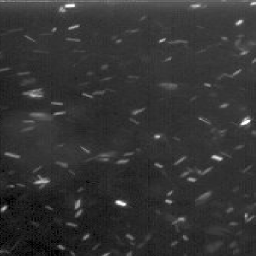
\includegraphics[width=.32\textwidth]{1_in}
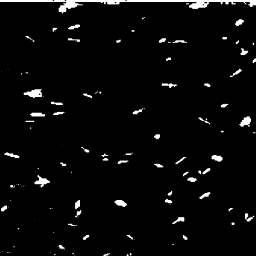
\includegraphics[width=.32\textwidth]{1_binarized}
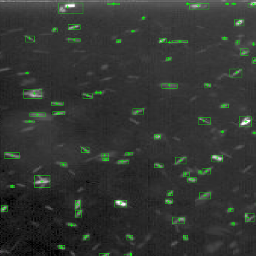
\includegraphics[width=.32\textwidth]{1_out}
\end{card}
\vspace{-.5cm}
\begin{cardTiny}
Raw image - binary image - blobs marked on the original image.  
\end{cardTiny}
\end{frame}


\begin{frame}[label=real-13]{Real life is not like this}
\begin{multicols}{2}

\includegraphics[width=.49\textwidth]{background.png}
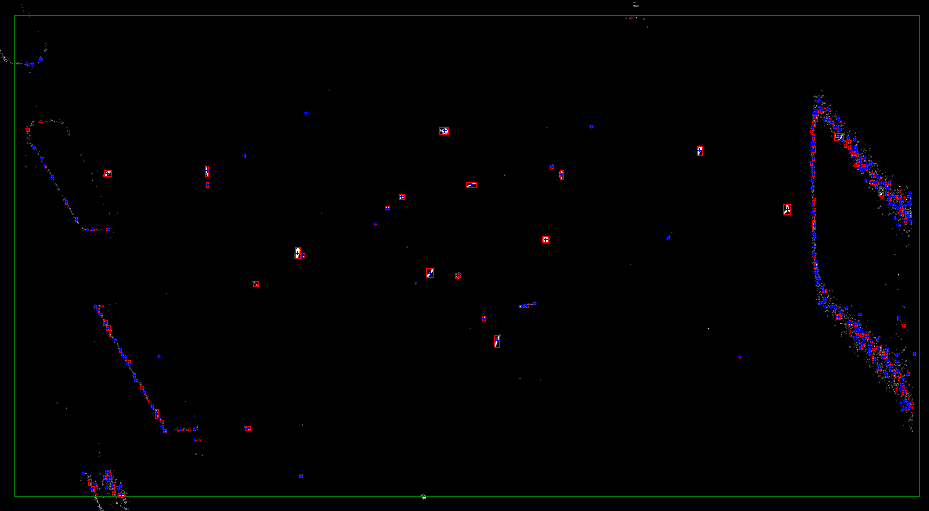
\includegraphics[width=.49\textwidth]{detection.png}
\end{multicols}
\begin{cardTiny}
Raw 3D-PTV image of the wind tunnel experiments: Background ->  binary image after background subtraction, and detection using a locally adaptive filter
\end{cardTiny}
\end{frame}

\begin{frame}[label=real-12]{We had to develop the know-how}
\centering\cardImg{1vision}{1\textwidth}
\end{frame}


\begin{frame}[label=real-11]{Image processing algorithm on FPGA}
\centering\cardImg{fig8}{1\textwidth}
% \begin{cardTiny} Diagram of the blob analysis algorithm. \end{cardTiny}
\end{frame}

\begin{frame}[label=real-10]{And its implementation on dedicated hardware}
\cardImg{1vision_blob_recorder_2}{1\textwidth}
% \cardImg{backside}{.25\textwidth}
\end{frame}

\begin{frame}[label=real-100]{The central concept diagram}
\centering
\cardImg[height=.8\textheight]{fig1.png}{\textwidth}
\end{frame}

%\end{document}
\topicFramePrimary{Some ideas on applications that could benefit from real-time 3D-PTV}
% \documentclass{beamer}
% \usepackage{graphicx}
% \usepackage{multicol}
% \setlength{\columnseprule}{1pt}
%
% \graphicspath{{./fig/}}
% \usetheme{material}
% %%%%%%%%%%%%%%%%%%%%%%%%%%%%%%%%%%%%%%%%%%%%%%%%%%%%%%%%%%%%%%%%%%%%%%%%%%%%%%
% \embedvideo{<poster or text>}{<video file (MP4+H264)>}
% \embedvideo*{...}{...}                     % auto-play
%%%%%%%%%%%%%%%%%%%%%%%%%%%%%%%%%%%%%%%%%%%%%%%%%%%%%%%%%%%%%%%%%%%%%%%%%%%%%%

\ExplSyntaxOn
\NewDocumentCommand\embedvideo{smm}{
  \group_begin:
  \leavevmode
  \tl_if_exist:cTF{file_\file_mdfive_hash:n{#3}}{
    \tl_set_eq:Nc\video{file_\file_mdfive_hash:n{#3}}
  }{
    \IfFileExists{#3}{}{\GenericError{}{File~`#3'~not~found}{}{}}
    \pbs_pdfobj:nnn{}{fstream}{{}{#3}}
    \pbs_pdfobj:nnn{}{dict}{
      /Type/Filespec/F~(#3)/UF~(#3)
      /EF~<</F~\pbs_pdflastobj:>>
    }
    \tl_set:Nx\video{\pbs_pdflastobj:}
    \tl_gset_eq:cN{file_\file_mdfive_hash:n{#3}}\video
  }
  %
  \pbs_pdfobj:nnn{}{dict}{
    /Type/RichMediaInstance/Subtype/Video
    /Asset~\video
    /Params~<</FlashVars (
      source=#3&
      skin=SkinOverAllNoFullNoCaption.swf&
      skinAutoHide=true&
      skinBackgroundColor=0x5F5F5F&
      skinBackgroundAlpha=0
    )>>
  }
  %
  \pbs_pdfobj:nnn{}{dict}{
    /Type/RichMediaConfiguration/Subtype/Video
    /Instances~[\pbs_pdflastobj:]
  }
  %
  \pbs_pdfobj:nnn{}{dict}{
    /Type/RichMediaContent
    /Assets~<<
      /Names~[(#3)~\video]
    >>
    /Configurations~[\pbs_pdflastobj:]
  }
  \tl_set:Nx\rmcontent{\pbs_pdflastobj:}
  %
  \pbs_pdfobj:nnn{}{dict}{
    /Activation~<<
      /Condition/\IfBooleanTF{#1}{PV}{XA}
      /Presentation~<</Style/Embedded>>
    >>
    /Deactivation~<</Condition/PI>>
  }
  %
  \hbox_set:Nn\l_tmpa_box{#2}
  \tl_set:Nx\l_box_wd_tl{\dim_use:N\box_wd:N\l_tmpa_box}
  \tl_set:Nx\l_box_ht_tl{\dim_use:N\box_ht:N\l_tmpa_box}
  \tl_set:Nx\l_box_dp_tl{\dim_use:N\box_dp:N\l_tmpa_box}
  \pbs_pdfxform:nnnnn{1}{1}{}{}{\l_tmpa_box}
  %
  \pbs_pdfannot:nnnn{\l_box_wd_tl}{\l_box_ht_tl}{\l_box_dp_tl}{
    /Subtype/RichMedia
    /BS~<</W~0/S/S>>
    /Contents~(embedded~video~file:#3)
    /NM~(rma:#3)
    /AP~<</N~\pbs_pdflastxform:>>
    /RichMediaSettings~\pbs_pdflastobj:
    /RichMediaContent~\rmcontent
  }
  \phantom{#2}
  \group_end:
}
\ExplSyntaxOff
%
%% \newlength{\wdth}
%
%% \newcommand{\strike}[1]{\settowidth{\wdth}{#1}\rlap{\rule[.5ex]{\wdth}{.4pt}}#1}
%
%
%\begin{document}

% %%%%%%%%%%%%%%%%%%%%%%%%%%%%%%%%%%%%%%%%%%%%%%%%%%%%%%%%%%%%%%%%%%%%%%%%%%%%%%
% \embedvideo{<poster or text>}{<video file (MP4+H264)>}
% \embedvideo*{...}{...}                     % auto-play
%%%%%%%%%%%%%%%%%%%%%%%%%%%%%%%%%%%%%%%%%%%%%%%%%%%%%%%%%%%%%%%%%%%%%%%%%%%%%%

\ExplSyntaxOn
\NewDocumentCommand\embedvideo{smm}{
  \group_begin:
  \leavevmode
  \tl_if_exist:cTF{file_\file_mdfive_hash:n{#3}}{
    \tl_set_eq:Nc\video{file_\file_mdfive_hash:n{#3}}
  }{
    \IfFileExists{#3}{}{\GenericError{}{File~`#3'~not~found}{}{}}
    \pbs_pdfobj:nnn{}{fstream}{{}{#3}}
    \pbs_pdfobj:nnn{}{dict}{
      /Type/Filespec/F~(#3)/UF~(#3)
      /EF~<</F~\pbs_pdflastobj:>>
    }
    \tl_set:Nx\video{\pbs_pdflastobj:}
    \tl_gset_eq:cN{file_\file_mdfive_hash:n{#3}}\video
  }
  %
  \pbs_pdfobj:nnn{}{dict}{
    /Type/RichMediaInstance/Subtype/Video
    /Asset~\video
    /Params~<</FlashVars (
      source=#3&
      skin=SkinOverAllNoFullNoCaption.swf&
      skinAutoHide=true&
      skinBackgroundColor=0x5F5F5F&
      skinBackgroundAlpha=0
    )>>
  }
  %
  \pbs_pdfobj:nnn{}{dict}{
    /Type/RichMediaConfiguration/Subtype/Video
    /Instances~[\pbs_pdflastobj:]
  }
  %
  \pbs_pdfobj:nnn{}{dict}{
    /Type/RichMediaContent
    /Assets~<<
      /Names~[(#3)~\video]
    >>
    /Configurations~[\pbs_pdflastobj:]
  }
  \tl_set:Nx\rmcontent{\pbs_pdflastobj:}
  %
  \pbs_pdfobj:nnn{}{dict}{
    /Activation~<<
      /Condition/\IfBooleanTF{#1}{PV}{XA}
      /Presentation~<</Style/Embedded>>
    >>
    /Deactivation~<</Condition/PI>>
  }
  %
  \hbox_set:Nn\l_tmpa_box{#2}
  \tl_set:Nx\l_box_wd_tl{\dim_use:N\box_wd:N\l_tmpa_box}
  \tl_set:Nx\l_box_ht_tl{\dim_use:N\box_ht:N\l_tmpa_box}
  \tl_set:Nx\l_box_dp_tl{\dim_use:N\box_dp:N\l_tmpa_box}
  \pbs_pdfxform:nnnnn{1}{1}{}{}{\l_tmpa_box}
  %
  \pbs_pdfannot:nnnn{\l_box_wd_tl}{\l_box_ht_tl}{\l_box_dp_tl}{
    /Subtype/RichMedia
    /BS~<</W~0/S/S>>
    /Contents~(embedded~video~file:#3)
    /NM~(rma:#3)
    /AP~<</N~\pbs_pdflastxform:>>
    /RichMediaSettings~\pbs_pdflastobj:
    /RichMediaContent~\rmcontent
  }
  \phantom{#2}
  \group_end:
}
\ExplSyntaxOff

\section{Applications}
\topicFramePrimary{Examples of applications that benefit from real-time 3D-PTV}

\begin{frame}[label=app-1]
\frametitle{Real-time flow information is beneficial in applications}
\begin{itemize}
	\item Time-varying on slow time scales
    \item Unpredictable start and duration 
    \item Irreproducible or expensive % add suction feeding stuff, ceramic particle release stuff, rupture and breakage
	\item Control of the flow-dependent process, or control the flow % add wind turbine stuff
    \item Mobile systems, field experiments
    \item Harsh environments, remote operation
\end{itemize}
\end{frame}

\begin{frame}[label=app-2]{Particle motion due to pressure change in loadlocks}
\centering\cardImg{lab1}{\textwidth}
\end{frame}

\begin{frame}[label=app-3]{We can leave the lab}
\begin{multicols}{2}
    \cardImg{ldc3}{.49\textwidth}
    \cardImg{ldc_splitter}{.49\textwidth}
\end{multicols}
\end{frame}


\begin{frame}[label=iibr-4]{3D flow inside canopy in a large scale Environmental Wind Tunnel}
\begin{columns}
\column{0.5\textwidth}
    \cardImg{wind_tunnel_photo_1}{1\textwidth}
%\end{frame}
%\begin{frame}[label=iibr-5]{We are ready for the Environmental Wind Tunnel}
\column{0.5\textwidth}
    \cardImg{ptv_wind_tunnel_photo1}{1\textwidth}
\end{columns}
\end{frame}

\begin{frame}[label=app-19]{Flow inside the canopy \href{https://www.dropbox.com/s/9x43i2uk9q38fho/flow_inside_laser.mp4?raw=1}{video}}
    \centering
    \embedvideo{\cardImg{flow_snapshot_inside.jpg}{.9\textwidth}}{video/flow_inside_laser.mp4}
\end{frame}
    

\begin{frame}[label=app-12]{The whole system can slide or rotate}
    \cardImg{sliding_ptv.jpg}{.9\textwidth}
    \begin{cardTiny} 
        Walpot et al. Meas. Sci. Tech. 2006. TU/e
    \end{cardTiny}
\end{frame}
    

\begin{frame}[label=app-6]{Rotation table experiments, \href{https://www.dropbox.com/s/933wsb9xdahbyi9/rotation.mp4?raw=1}{ETH Zurich}}
    \embedvideo{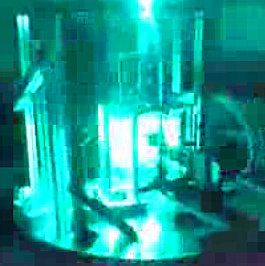
\includegraphics[width=0.8\textwidth]{fig/rotation.jpg}}{video/rotation.mp4}
\end{frame}
    
  
\begin{frame}[label=app-7]{Microgravity applications: remote and \href{https://www.dropbox.com/s/59ophf177gcfjzq/boiling_microgravity.mp4?raw=1}{difficult to control}}   
    % \begin{columns}
    % \column{.4\textwidth}
    %     \cardImg{microgravity}{\linewidth}
    % \column{.7\textwidth}
    \centering
    \embedvideo{\cardImg{space_3d_ptv}{.8\textwidth}}{video/boiling_microgravity.mp4}    
        
%    \end{columns}
\end{frame}


% \begin{frame}[label=app-11]{Real-time is easier with a single camera with a four-view splitter}
%     \centering\cardImg{ldc_splitter}{0.8\textwidth}
%     \embedvideo{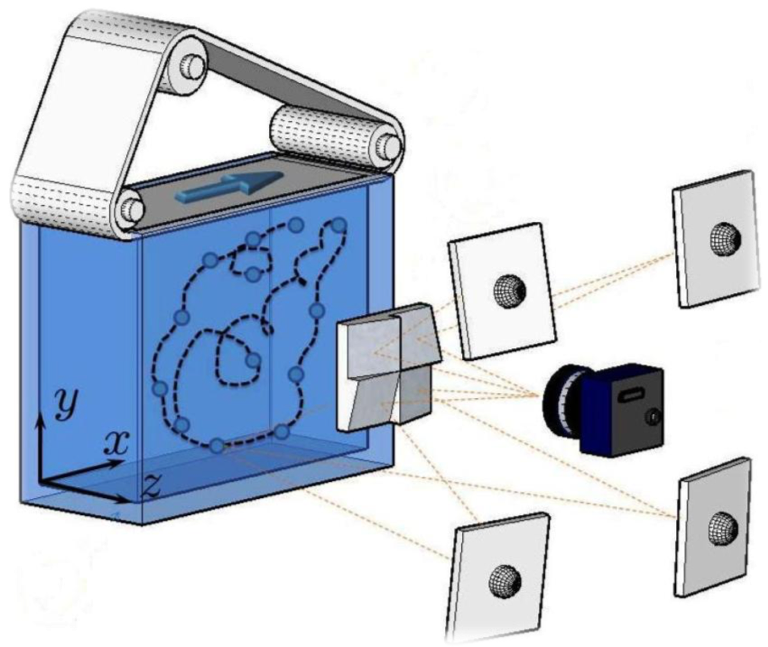
\includegraphics[width=\textwidth]{ldc_splitter}}{video/splitter_short.mp4}
%     % \begin{cardTiny} A high speed camera with a four-view optical system \end{cardTiny}
% \end{frame}

    
\begin{frame}[label=app-8]{An example from Chamorro's group}
    \centering\cardImg{kim/setup.png}{.9\textwidth}
\end{frame}
    
\begin{frame}[label=app-9]{Four view splitter \href{https://www.dropbox.com/s/h6g8d373lxgkqv8/Video1a.mp4?raw=1}{video}}
    \embedvideo{
\includegraphics[width=.8\textwidth]{fig/kim/4views.png}}{fig/kim/Video1a.mp4}
\end{frame}
    
% \begin{frame}[label=app-10]{You can get very dense result: turbulent jet}
%     \centering\cardImg{kim/jet.png}{\textwidth}
% \end{frame}

\begin{frame}[label=app-10b]{You can adjust 3D-PTV to microflows, using defocusing, scanning, photogrammetry}
\begin{center}
\begin{columns}
\column{.7\textwidth}
	\cardImg{kim/micro_3dptv.png}{\textwidth}
\column{.3\textwidth}
	\cardImg{kim/micro_3dptv_result.png}{\textwidth}
\end{columns}
\end{center}
\end{frame}


\begin{frame}[label=app-13]{Remote application and harsh environment: MRI + 3D-PTV}
    \begin{columns}
    \column{.5\textwidth}
        \cardImg{mri2}{.75\textwidth}
        \cardImg{mri3}{.75\textwidth}
    \column{.5\textwidth}
        \centering\cardImg{mri1}{\textwidth}
    \end{columns}
\end{frame}

\begin{frame}[label=app-14]{Biomedical applications: moving boundaries + complex geometries, \href{https://www.dropbox.com/s/p1xnc7mefoqboti/aorta_rigid.mp4?dl=0}{ETH Zurich}}
\embedvideo{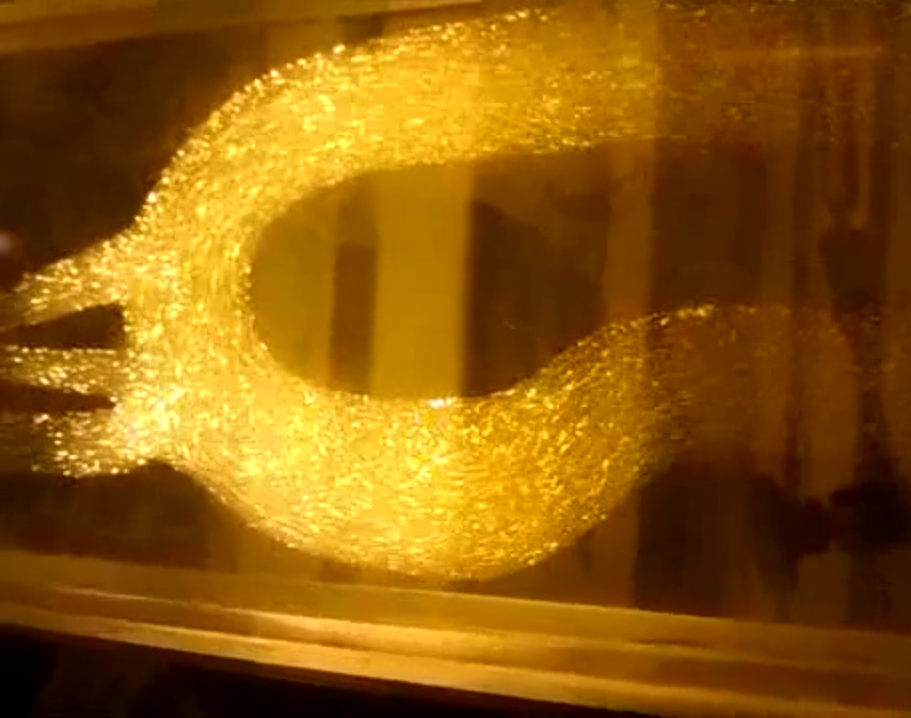
\includegraphics[width=\textwidth]{fig/aorta.png}}{video/aorta_rigid.mp4}
    \cardImg{aorta}{.9\textwidth}
\end{frame}

\begin{frame}[label=app-15]{Cerebrospinal fluid project -- \href{https://idsc.ethz.ch/research-guzzella-onder/research-projects/ProjectArchive/csf-biothermofluidics.html}{ETH Zurich}}
\embedvideo{\cardImg{brain}{\textwidth}}{video/brain.mp4}
\end{frame}
    
% \begin{frame}[label=iibr-16]{Camera system and laser}
%     \begin{multicols}{2}
%     \centering
%     \cardImg{camera_system_laser.jpg}{0.49\textwidth}
%     \cardImg{calibration_in_laser.jpg}{.49\textwidth}
%     \end{multicols}
%     \begin{cardTiny}
%     Four cameras point into the measurement location, as seen from the test section inside the tunnel, and the calibration target is mounted on the traverse arm.
%     \end{cardTiny}
% \end{frame}
    
%     %
% \begin{frame}[label=iibr-17]{Camera system and laser}
%     \begin{multicols}{2}
%     \centering\cardImg{img1.jpg}{.49\textwidth}
%     \cardImg{camera_system_laser.jpg}{0.49\textwidth}
%     \end{multicols}
% \end{frame}
    
    % \begin{frame}{Pressurized air seeding devices}
    % \cardImg{seeding_sources_2.jpg}{0.9\textwidth}
    % \end{frame}
    
    % \begin{frame}{Seeding material}
    % \centering\cardImg{SiO2_003}{0.75\textwidth}
    % \end{frame}
    
    
    % \subsection{3D Particle Tracking Velocimetry}
    
    %\begin{frame}
    %\centering\cardImg{volumes.png}{.6\textwidth}
    %\begin{cardTiny}
    %Representation in the isometric view of the measurement sub-volumes within and above the canopy layer. The arrow points in the streamwise direction.
    %\end{cardTiny}
    %\end{frame}
    
    
    % \begin{frame}[label=app-18]{Flow above the canopy}
    % \centering
    % \cardImg{flow_snapshot_above.jpg}{.9\textwidth}
    % \end{frame}
    
    % \begin{frame}[label=app-19]{Flow inside the canopy}
    % \centering
    % \cardImg{flow_snapshot_inside.jpg}{.9\textwidth}
    % \end{frame}
    
    % \begin{frame}[label=app-10]{\href{./fig/flow_inside_laser.mp4}{Video clip}}
    % \centering\cardImg{flow_snapshot_inside.jpg}{\textwidth}
    % \end{frame}
    
%    
%    

%    
%    
% \begin{frame}[label=app-21]{Take it to the space -- video credit: \href{https://www.dropbox.com/s/59ophf177gcfjzq/boiling_microgravity.mp4?raw=1}{ESA}}
%     %\cardImg{maser_8}{0.3\textwidth}
%     \embedvideo{\cardImg{space_3d_ptv}{0.8\textwidth}}{video/boiling_microgravity.mp4}
%     \begin{cardTiny}
%     Design and calibration of a four-headed camera for use in microgravity research, Willneff and Maas, ETH Zurich
%     \end{cardTiny}
% \end{frame}
    

\begin{frame}[label=app-22]
    \frametitle{Suction feeding events, courtesy of \href{https://www.dropbox.com/s/wcytdkxuxxvn4q0/fish_feeding.mp4?raw=1}{Prof. Roi Holzman, TAU}}
    \embedvideo{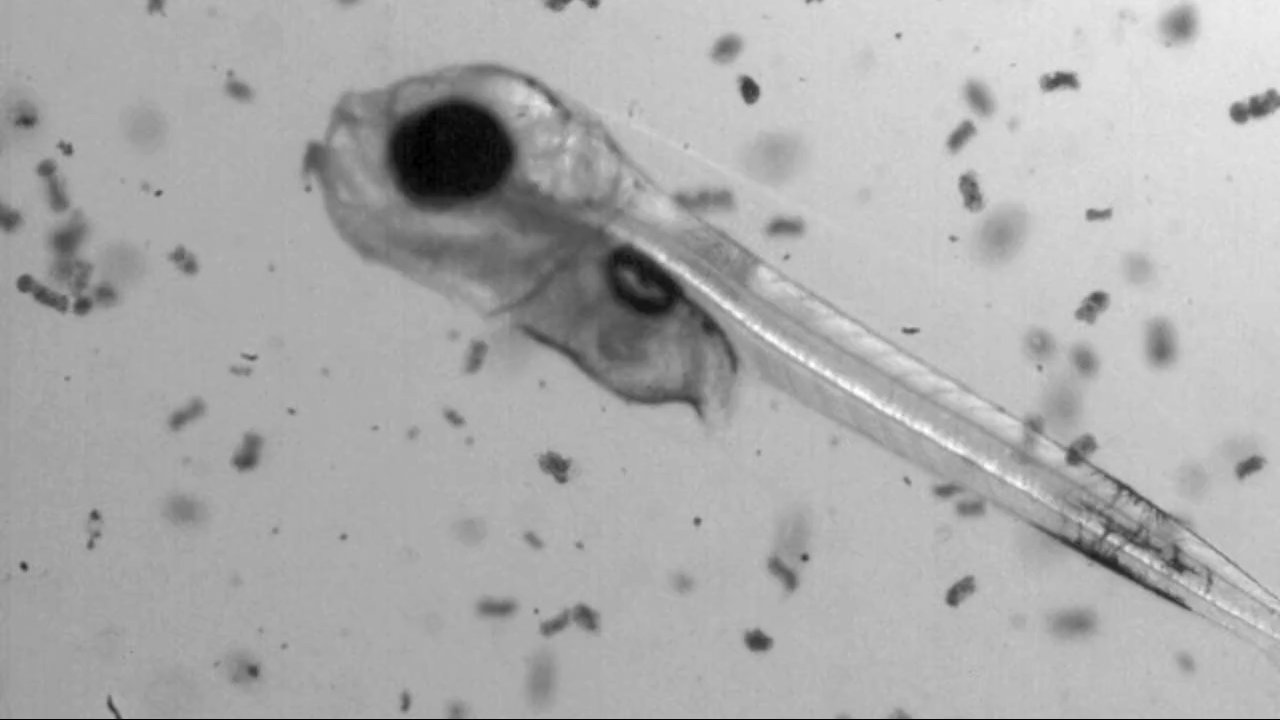
\includegraphics[width=\textwidth]{fig/fish_feeding.png}}{video/fish_feeding.mp4}
    %or this great video from Monterey Bay Aquarium 
    %
    %https://www.youtube.com/watch?v=umTqQSzKRmA    
\end{frame}
    
\begin{frame}[label=app-23]
    \frametitle{Flamingo underwater feeding -- \href{https://www.dropbox.com/s/ic0l5npzon834l9/flamingo.mp4?raw=1}{San Diego Zoo}}
    % https://www.youtube.com/watch?v=-1BF2XqboOo
    \begin{center}
    \embedvideo{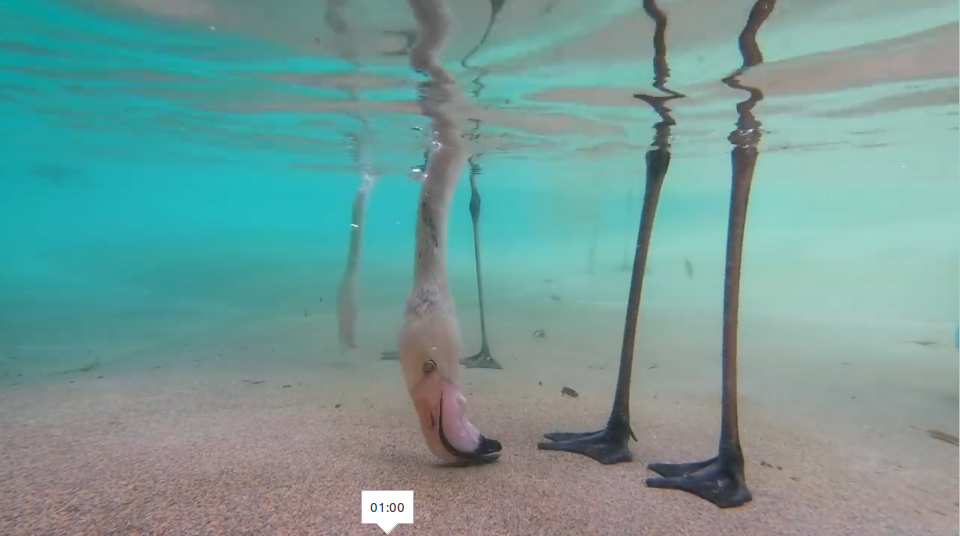
\includegraphics[width=\textwidth]{fig/flamingo.png}}{video/flamingo.mp4}
    \end{center}
\end{frame}
    
    %
    
\begin{frame}[label=app-24]
    \frametitle{Colloid aggregates breakage in extensional 3D flow, \href{https://www.dropbox.com/s/aufwfraotj5rll7/colloids1.mp4?raw=1}{ETH Zurich}}
    %https://pubs.acs.org/doi/10.1021/acs.langmuir.5b03804
\begin{center}
    \embedvideo{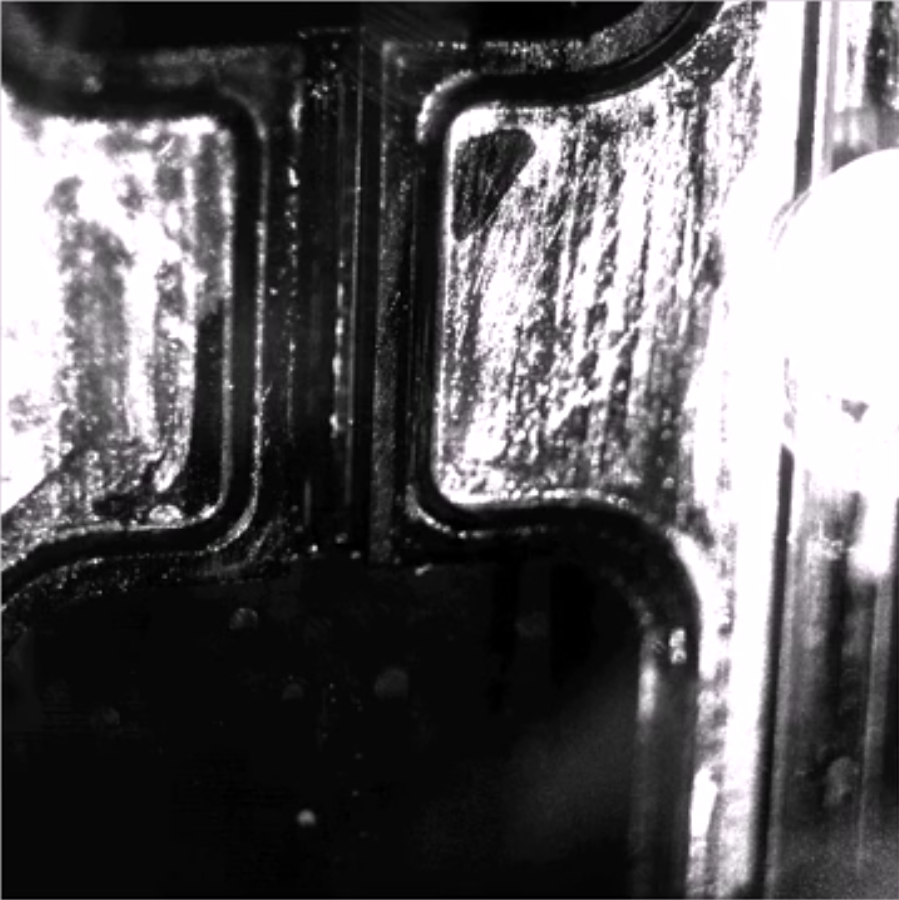
\includegraphics[width=\textwidth]{fig/colloids1.png}}{video/colloids1.mp4}
\end{center}    
\end{frame}
    
\begin{frame}[label=app-25]{Quantify colloid aggregates breakage in turbulence \href{https://www.dropbox.com/s/8cimpwfsukf11u2/colloids2.mp4?raw=1}{ETH Zurich}}
    %https://pubs.acs.org/doi/10.1021/acs.langmuir.5b03804
\begin{center}
    \embedvideo{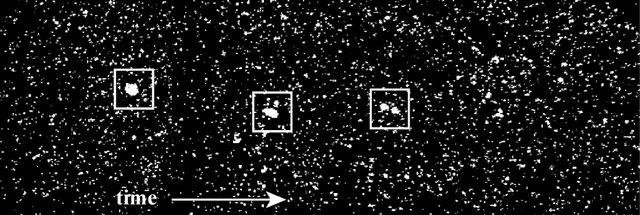
\includegraphics[width=\textwidth]{colloid_sequence.jpg}}{video/colloids2.mp4}
\end{center}       
\end{frame}
    
    
\begin{frame}[label=app-26]{Real-time vortex identification for wind turbine blade pitch control -- Caroline Braud}
    \begin{multicols*}{2}
    \cardImg{real_time_vortex_1}{.49\textwidth}
    \cardImg{real_time_vortex_2}{.49\textwidth}
    \end{multicols*}
\end{frame}
    
\begin{frame}[label=app-27]{Real-time sizing with 3D tracking -- Rayne Ramirez, Uni. Oslo}
  \begin{columns}
    \column{0.5\textwidth}
        \cardImg{drop-example}{\textwidth}
    \column{0.5\textwidth}
        \cardImg{drops}{\textwidth}
 \end{columns}
\end{frame}
    
\begin{frame}[label=app-28]{Fibers -- \href{https://www.dropbox.com/s/y5gf55qqeyq5ljr/fibers.mp4?raw=1}{Stefano Brizzolara, ETH Zurich}}
    % https://twitter.com/stebrizzo94/status/1525577322144976910?s=20
\begin{center}
    \embedvideo{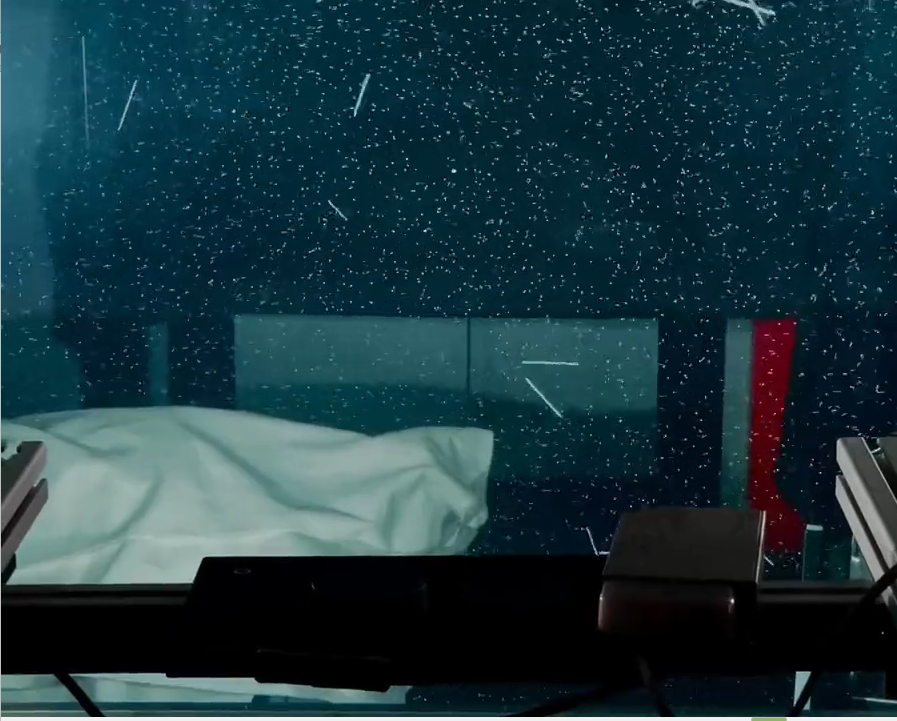
\includegraphics[height=0.8\textheight]{fibers.png}}{video/fibers.mp4}
\end{center}    
\end{frame}

\begin{frame}[label=app-29]{Microplastics in a vortex - \href{https://www.dropbox.com/s/in5ewv968dy9j3q/microplastics.mp4?raw=1}{Turbulence Structure Laboratory}}
    % Imaging‑based 3D particle tracking system forfield characterization ofparticle dynamics inatmospheric flows
    \embedvideo{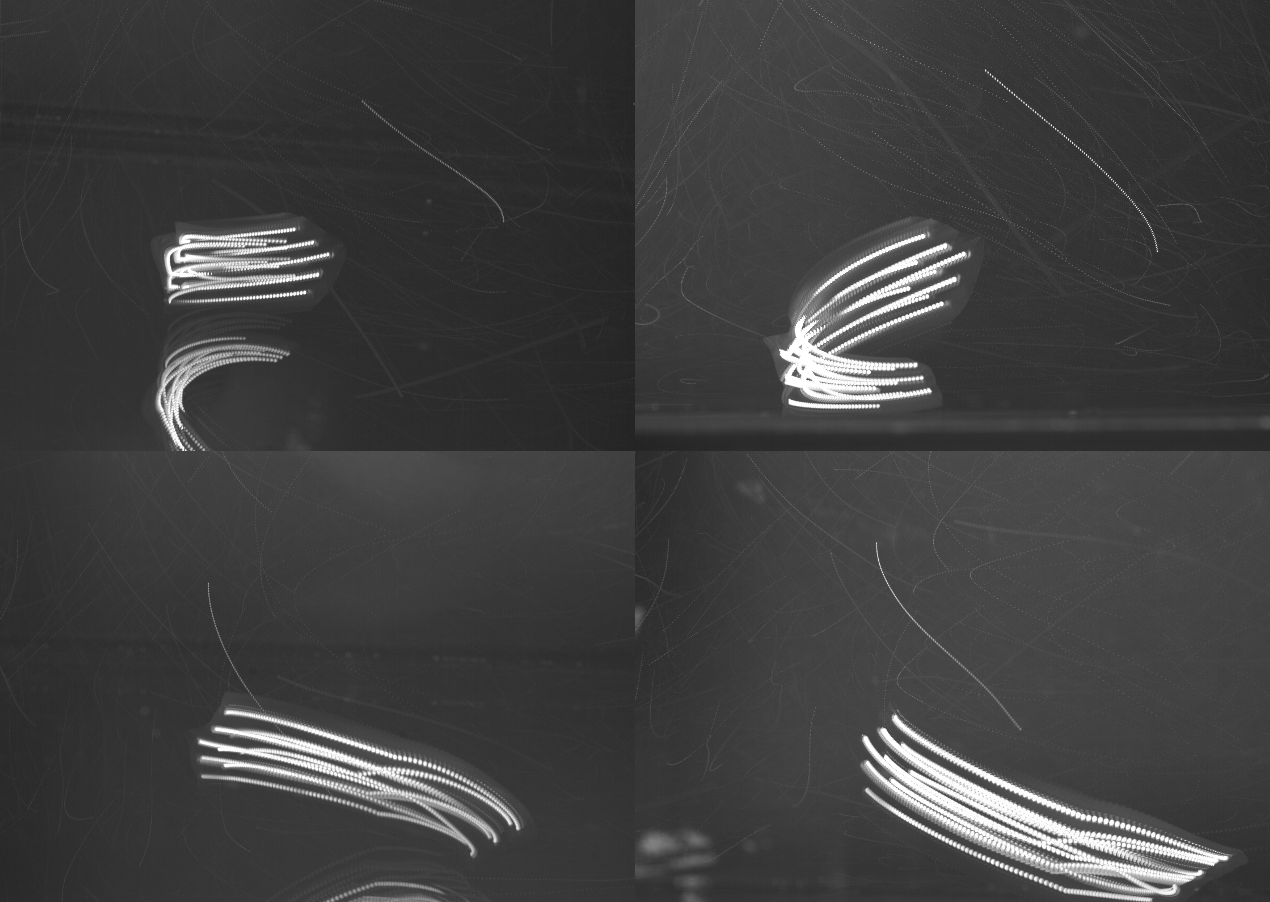
\includegraphics[height=\textheight]{trajects.png}}{video/microplastics2.mp4}\\
    Bristow et al. Exp. Fluids, 2023
\end{frame}

    
\begin{frame}[label=app-18a]{Multiphase flows - track both particles and flow, \href{}{inertial clustering}}
\begin{center}
    \embedvideo{\cardImg[height=.8\textheight]{two_phase_3dptv}
    {0.8\textwidth}}{video/twophase.mp4}
\end{center}
\end{frame}
    
    
\begin{frame}[label=app-30]{Drone vs turbulence - \href{https://www.dropbox.com/s/3lav5rf6s8su6f5/drone.mp4?raw=1}{University of Minnesota}}
    % Imaging‑based 3D particle tracking system forfield characterization ofparticle dynamics inatmospheric flows
    \begin{center}
    \embedvideo{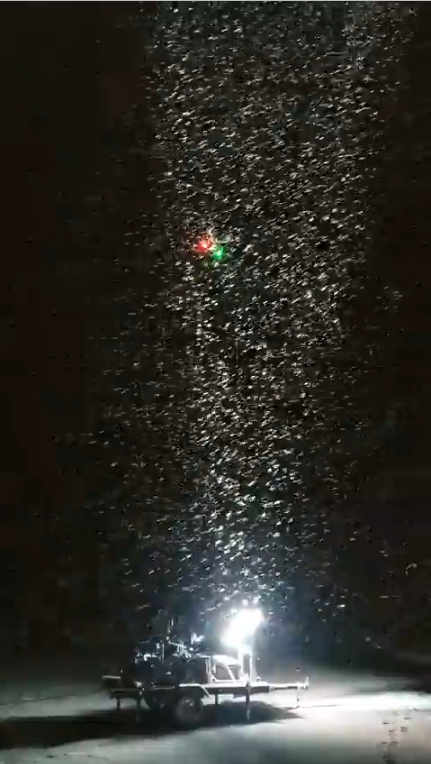
\includegraphics[height=0.8\textheight]{drone.png}}{video/drone.mp4}\\
    Bristow et al. Exp. Fluids, 2023
    \end{center}
\end{frame}
    
\begin{frame}[label=app-31a]{Soon we could do it using \href{https://www.dropbox.com/s/ckis9r6omd5y4fq/vuforia.mp4?raw=1}{AR/VR}}
    \centering 
    \embedvideo{\cardImg{mr_ptv_photo}{0.8\textwidth}}{video/vuforia.mp4}
    Chivers, T. Uni. Vermont, MSc Thesis, 2023 and Vuforia promotional video
\end{frame}

\begin{frame}[label=app-31b]{Real-time 3D-PTV is enabling technology for autonomous lab: \href{https://self-driving-lab-demo.readthedocs.io/en/latest/index.html}{self-driving-lab-demo.readthedocs.io}}
    \centering \cardImg[height=.75\textheight]{automatic_lab_concept}{\textwidth}
\end{frame}
        
    
% \begin{frame}[label=app-32]{Turbulent flow inside an urban canopy model at \href{https://www.dropbox.com/s/9x43i2uk9q38fho/flow_inside_laser.mp4?raw=1}{IIBR wind tunnel}}
%     \embedvideo{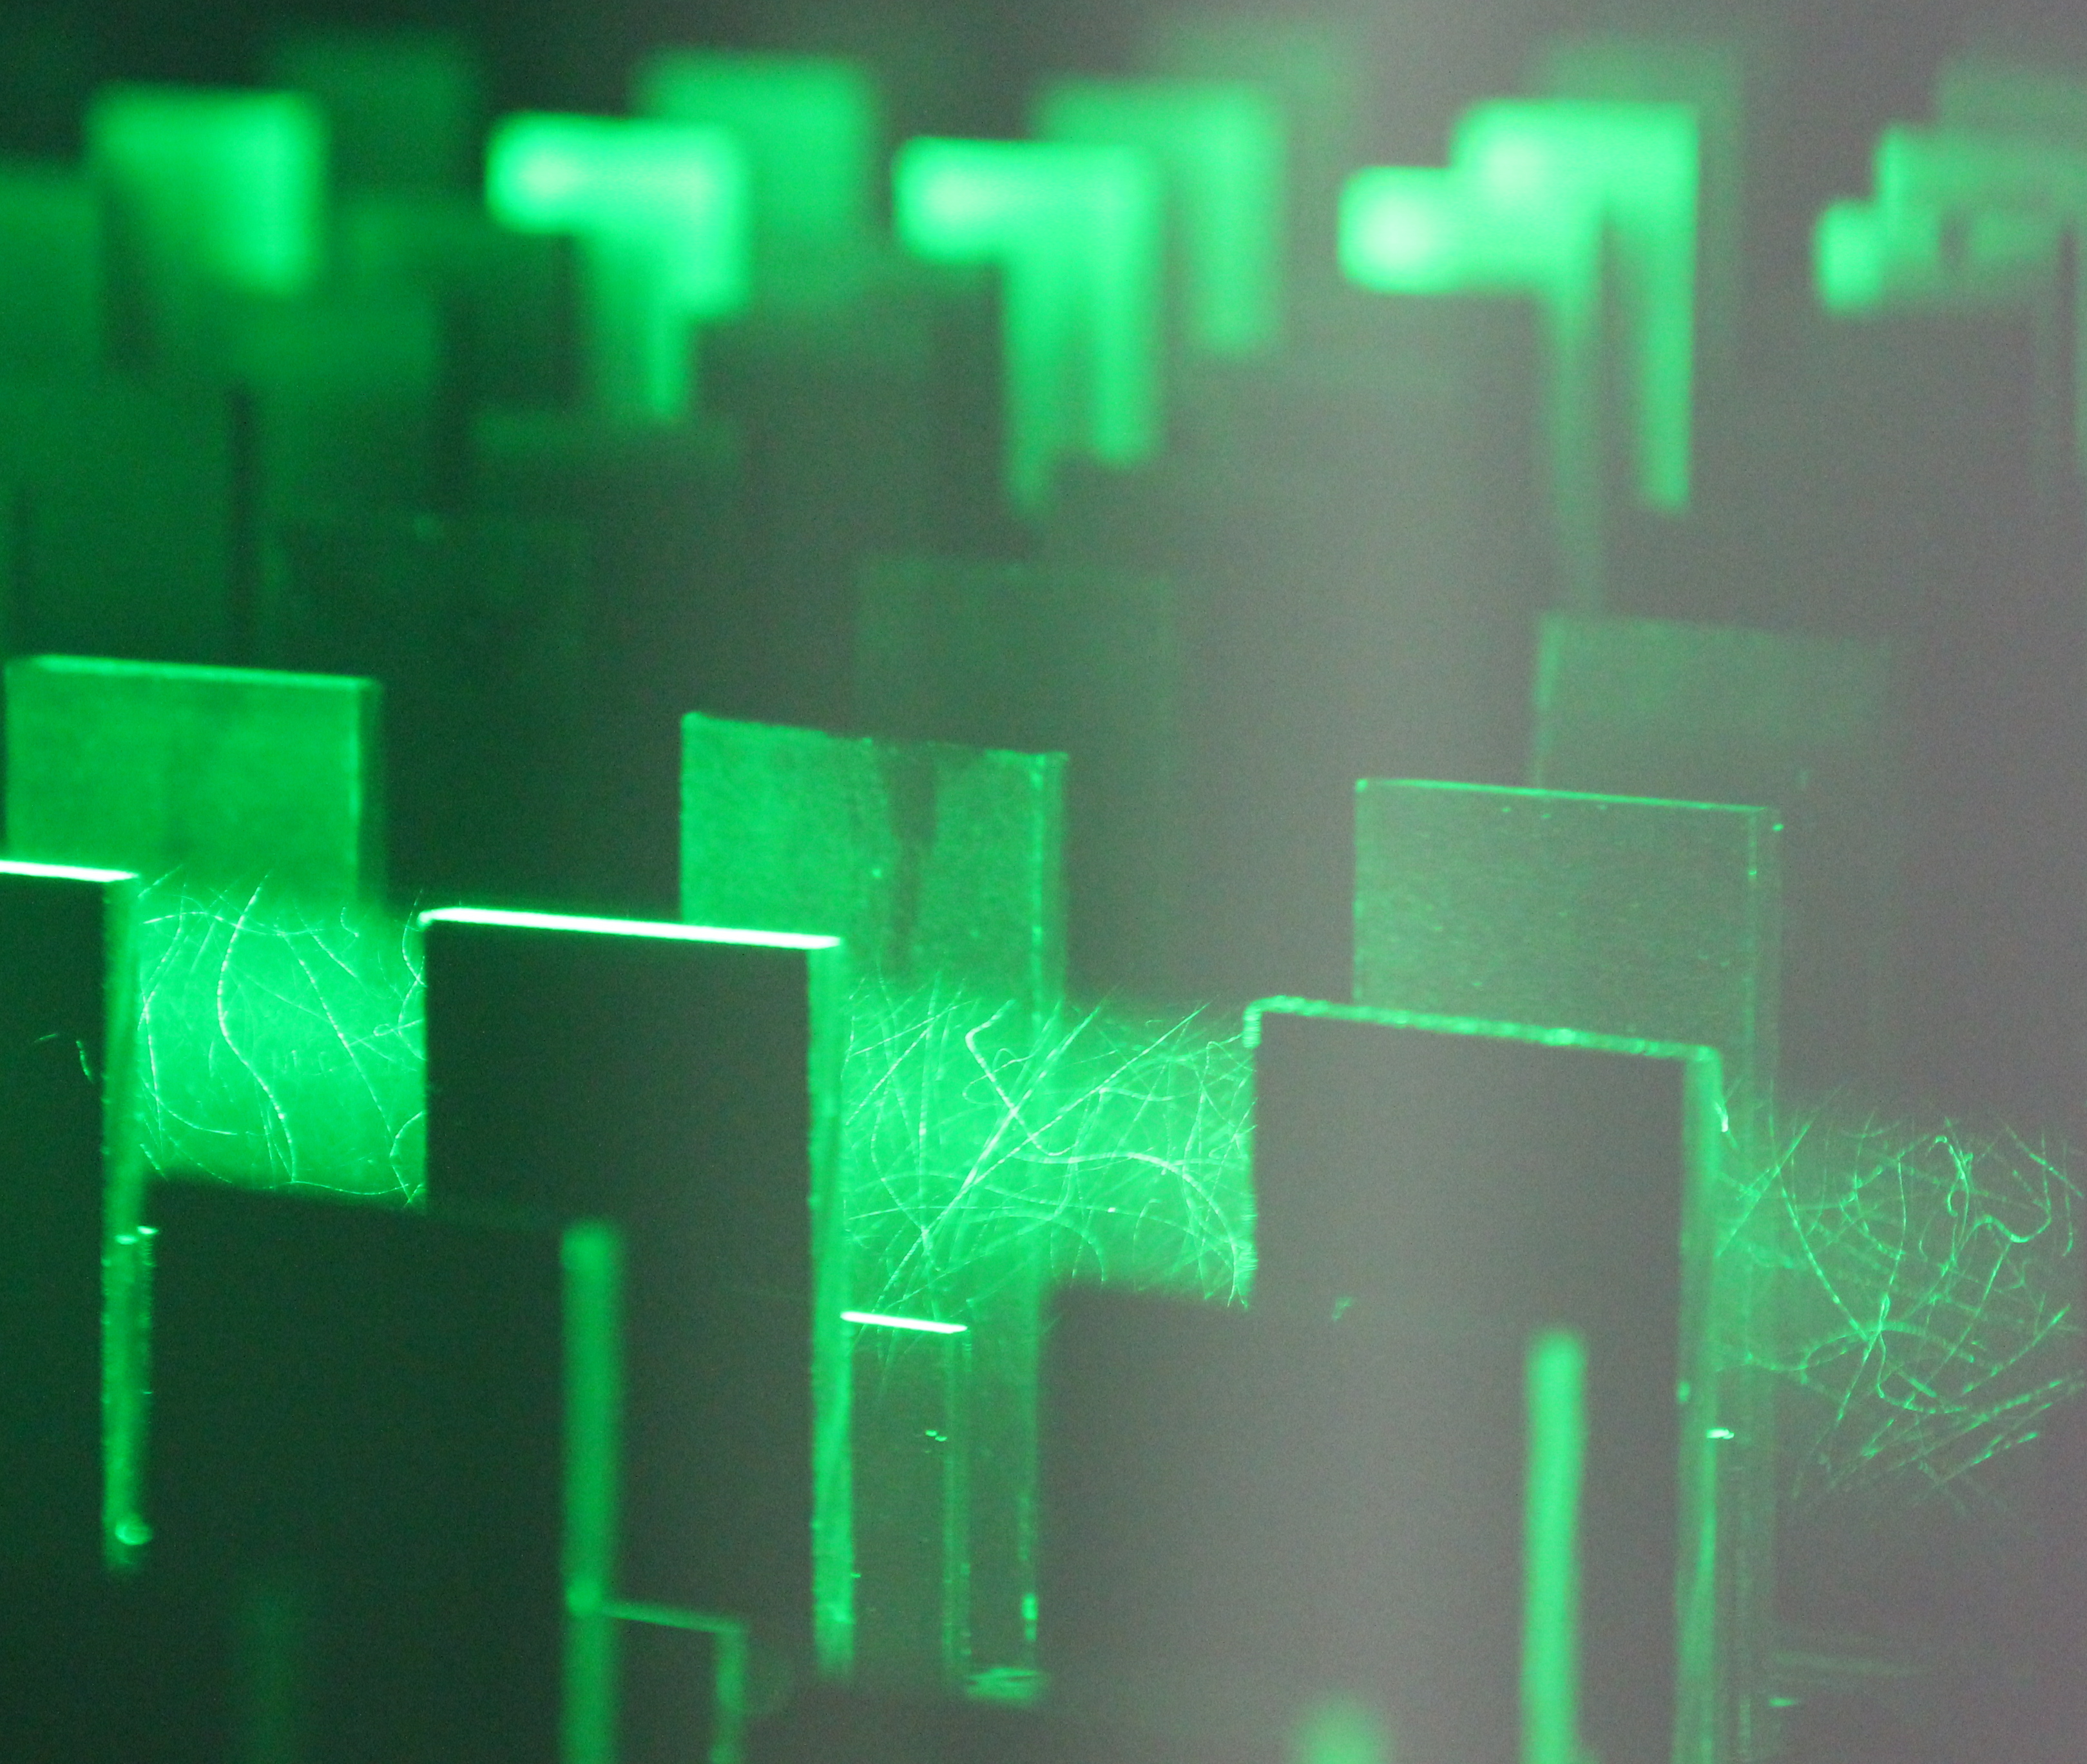
\includegraphics[width=\textwidth]{flow_snapshot_inside.jpg}}{video/flow_inside_laser.mp4}
% \end{frame}
%    

%\end{document}

\begin{frame}[label=app-20]{You could also do PIV on FPGA}
    \centering \cardImg[height=.75\textheight]{real_time_piv_fpga.png}{\textwidth}
    \begin{cardTiny}
    Real-time particle image velocimetry based on FPGA technology, Munoz et al. IEEE (2009)
    \end{cardTiny}
\end{frame}

    
\begin{frame}[label=app-17a]{But 3D-PTV can you give more insight in terms of 3D structure and turbulence}
    \begin{cardTiny} 
    This means we need  the \alert{full gradient tensor} along the particle trajectories:
    $\partial u_{i}/\partial x_{j}$ in space and time
    \end{cardTiny}
    \begin{multicols}{2}
    \centering
    \cardImg{moffatt2}{.49\textwidth}
    \cardImg{ptvgif}{.49\textwidth}
    \end{multicols}
\end{frame}


\section{Benefits of open source and open science}
\topicFramePrimary{It is important to work collectively and co-develop open-source software = sustainability}

\begin{frame}
\frametitle{Benefits of Open Source}
\begin{itemize}
\item Explain the benefits of developing real-time 3D-PTV as an open-source project, such as increased collaboration and sharing of knowledge.
\item Describe how the open-source approach has been successful in other scientific fields, such as software development and data science.
\item Outline some of the potential challenges of developing an open-source real-time 3D-PTV project and how they can be addressed.
\end{itemize}
\end{frame}


\begin{frame}{Open source software suite, all on Github}
\begin{itemize}
\item 
\includegraphics[width=0.5\textwidth]{openptv} \hspace{1em} library, `liboptv`, ANSI C
\item PyPTV GUI for {\em liboptv} in Python 
\includegraphics[width=.3\textwidth]{pyptv}
\item FlowTracks - trajectories database management (see Meller and Liberzon 2016)
\item BlobRecorder - proprietary hardware/customized software (see Shnapp et al. arxiv)
\end{itemize}
\end{frame}

	 
%\subsection{Post Processing}

\begin{frame}[label=opensource-1]{Open source software suite, all on Github}
\begin{itemize}
\item 
\includegraphics[width=0.5\textwidth]{openptv} \hspace{1em} library, `liboptv`, ANSI C
\item PyPTV GUI for {\em liboptv} in Python 
\includegraphics[width=.3\textwidth]{pyptv}
\item FlowTracks - trajectories database management (see Meller and Liberzon 2016)
\item BlobRecorder - proprietary hardware/customized software (see Shnapp et al. arxiv)
\end{itemize}
\end{frame}


\begin{frame}
\frametitle{Conclusions}
\begin{itemize}
\item Summarize the key points of the presentation and reiterate the importance of real-time 3D-PTV and the benefits of developing it as an open-source project.
\item Encourage audience members to become involved in real-time 3D-PTV research and development.
\item Deliver the message to industry professionals, research scientists, and graduate students that their participation in developing real-time 3D-PTV as an open-source project can lead to significant benefits for all involved, including improved collaboration, knowledge-sharing, and scientific advancements.
\end{itemize}
\end{frame}




\section{Summary and conclusions}\label{sec:summary}

\begin{frame}{Summary}
\begin{itemize}
\item Real-time imaging changed the 3D-PTV method and the way we think about it
\item Field experiments, webcam or Kinect-based, wind tunnel experiments, space station microgravity experiments are possible
\item Direct Lagrangian information in complex urban canopy flows is under analysis
\item Close coordination with the modeling efforts of Lagrangian dispersion or Lagrangian puff models
\end{itemize}
\end{frame}



\begin{frame}{Closing Thoughts}

Real-time 3D particle tracking velocimetry (3D-PTV) provides numerous advantages for fluid flow measurement and analysis, including:

\begin{itemize}
\item Immediate feedback on the velocity field
\item Faster decision-making
\item Improved accuracy and precision of measured data
\item Detailed insight into fluid dynamics
\item Real-time issue detection and troubleshooting
\end{itemize}

Real-time 3D-PTV is an invaluable tool for a wide range of applications, from fundamental fluid dynamics research to industrial process optimization and safety-critical applications.

\bigskip
Thank you for your attention!

\end{frame}

% \begin{frame}{Thank you for your attention}
% \cardImg{photo}{\textwidth}
% \end{frame}



\subsection{Credits}
\topicFramePrimary{Credits}

\begin{frame}[label=credit-1a]{The credit goes to the collaborators }
\begin{multicols}{2}
\centering
\cardImg{group_photo.jpg}{.49\textwidth} \cardImg{calibration_team.jpg}{0.49\textwidth}
\cardImg{sabrina_caliper.jpg}{.49\textwidth}\cardImg{meny_sabrina.jpg}{0.49\textwidth}
\end{multicols}
\end{frame}
%
\begin{frame}[label=credit-2]
\begin{card}[Israeli Institute for Biological Research]
Eyal Fattal, Yardena Raviv, Valery Babin, Mordechai Hotoveli, David Perry
\end{card}
\begin{card}[TAU]
Ron Shnapp, Meny Kon, Grigori Gulitski, Sabrina Shlain
\end{card}
\begin{card}[Funding]
Israel Science Foundation, PAZY Grant, Metro 450 grant
\end{card}
\end{frame}
%

\subsection{Credits}

\begin{frame}[label=credit-1]{The credit goes to the collaborators }
\begin{multicols}{2}
\centering
\cardImg{group_photo.jpg}{.49\textwidth} \cardImg{calibration_team.jpg}{0.49\textwidth}
\cardImg{sabrina_caliper.jpg}{.49\textwidth}\cardImg{meny_sabrina.jpg}{0.49\textwidth}
\end{multicols}
\end{frame}
%
\begin{frame}[label=credit-2]
\begin{card}[Israeli Institute for Biological Research]
Eyal Fattal, Yardena Raviv, Valery Babin, Mordechai Hotoveli, David Perry
\end{card}
\begin{card}[TAU]
Ron Shnapp, Meny Kon, Grigori Gulitski, Sabrina Shlain
\end{card}
\begin{card}[Funding]
Israel Science Foundation, PAZY Grant, Metro 450 grant
\end{card}
\end{frame}
%

% \begin{frame}[label=ron]
% \frametitle{We start with a happy end story}
% \cardImg{Ron.jpg}{0.8\textwidth}
% \begin{cardTiny}
% Ron Shnapp is a faculty at the Ben Gurion University, but it could turn out differently. 
% \end{cardTiny}
% \end{frame}

\begin{frame}{Take-home message}
\begin{itemize}
\item Customized real-time image analysis on FPGA can be implemented for long-recording, high-speed 3D-PTV
\item New developments change a paradigm about 3D-PTV: from the laboratory, table-top experiments to wind tunnels and field experiments
\item Instead of dense field representation (TomoPIV, Shake the box),  you can obtain an unprecedented data set of of Lagrangian trajectories, along with Lagrangian velocity and material derivative. 
\end{itemize}

\begin{cardTiny}\href{https://www.nature.com/articles/s41598-019-43555-2}{Details are in ``Extended 3D-PTV ...'' by Shnapp et al. Sci. Rep.}
\end{cardTiny}

\end{frame}
%

%
%%\begin{frame}{Lagrangian to Eulerian post-processing}
%%\centering\cardImg{voxel1}{.6\textwidth}
%%\end{frame}
%

	 
%\subsection{Post Processing}



\begin{frame}{Take-home message}
\begin{itemize}
\item Customized real-time image analysis on FPGA can be implemented for long-recording, high-speed 3D-PTV
\item New developments change a paradigm about 3D-PTV: from the laboratory, table-top experiments to wind tunnels and field experiments
\item Instead of dense field representation (TomoPIV, Shake the box),  you can obtain an unprecedented data set of of Lagrangian trajectories, along with Lagrangian velocity and material derivative. 
\end{itemize}
\end{frame}

\begin{frame}{Thanks for your attention \href{https://www.dropbox.com/s/resn98zu5l7vtty/real_time_3dptv.mp4?raw=1}{clip}}
\embedvideo{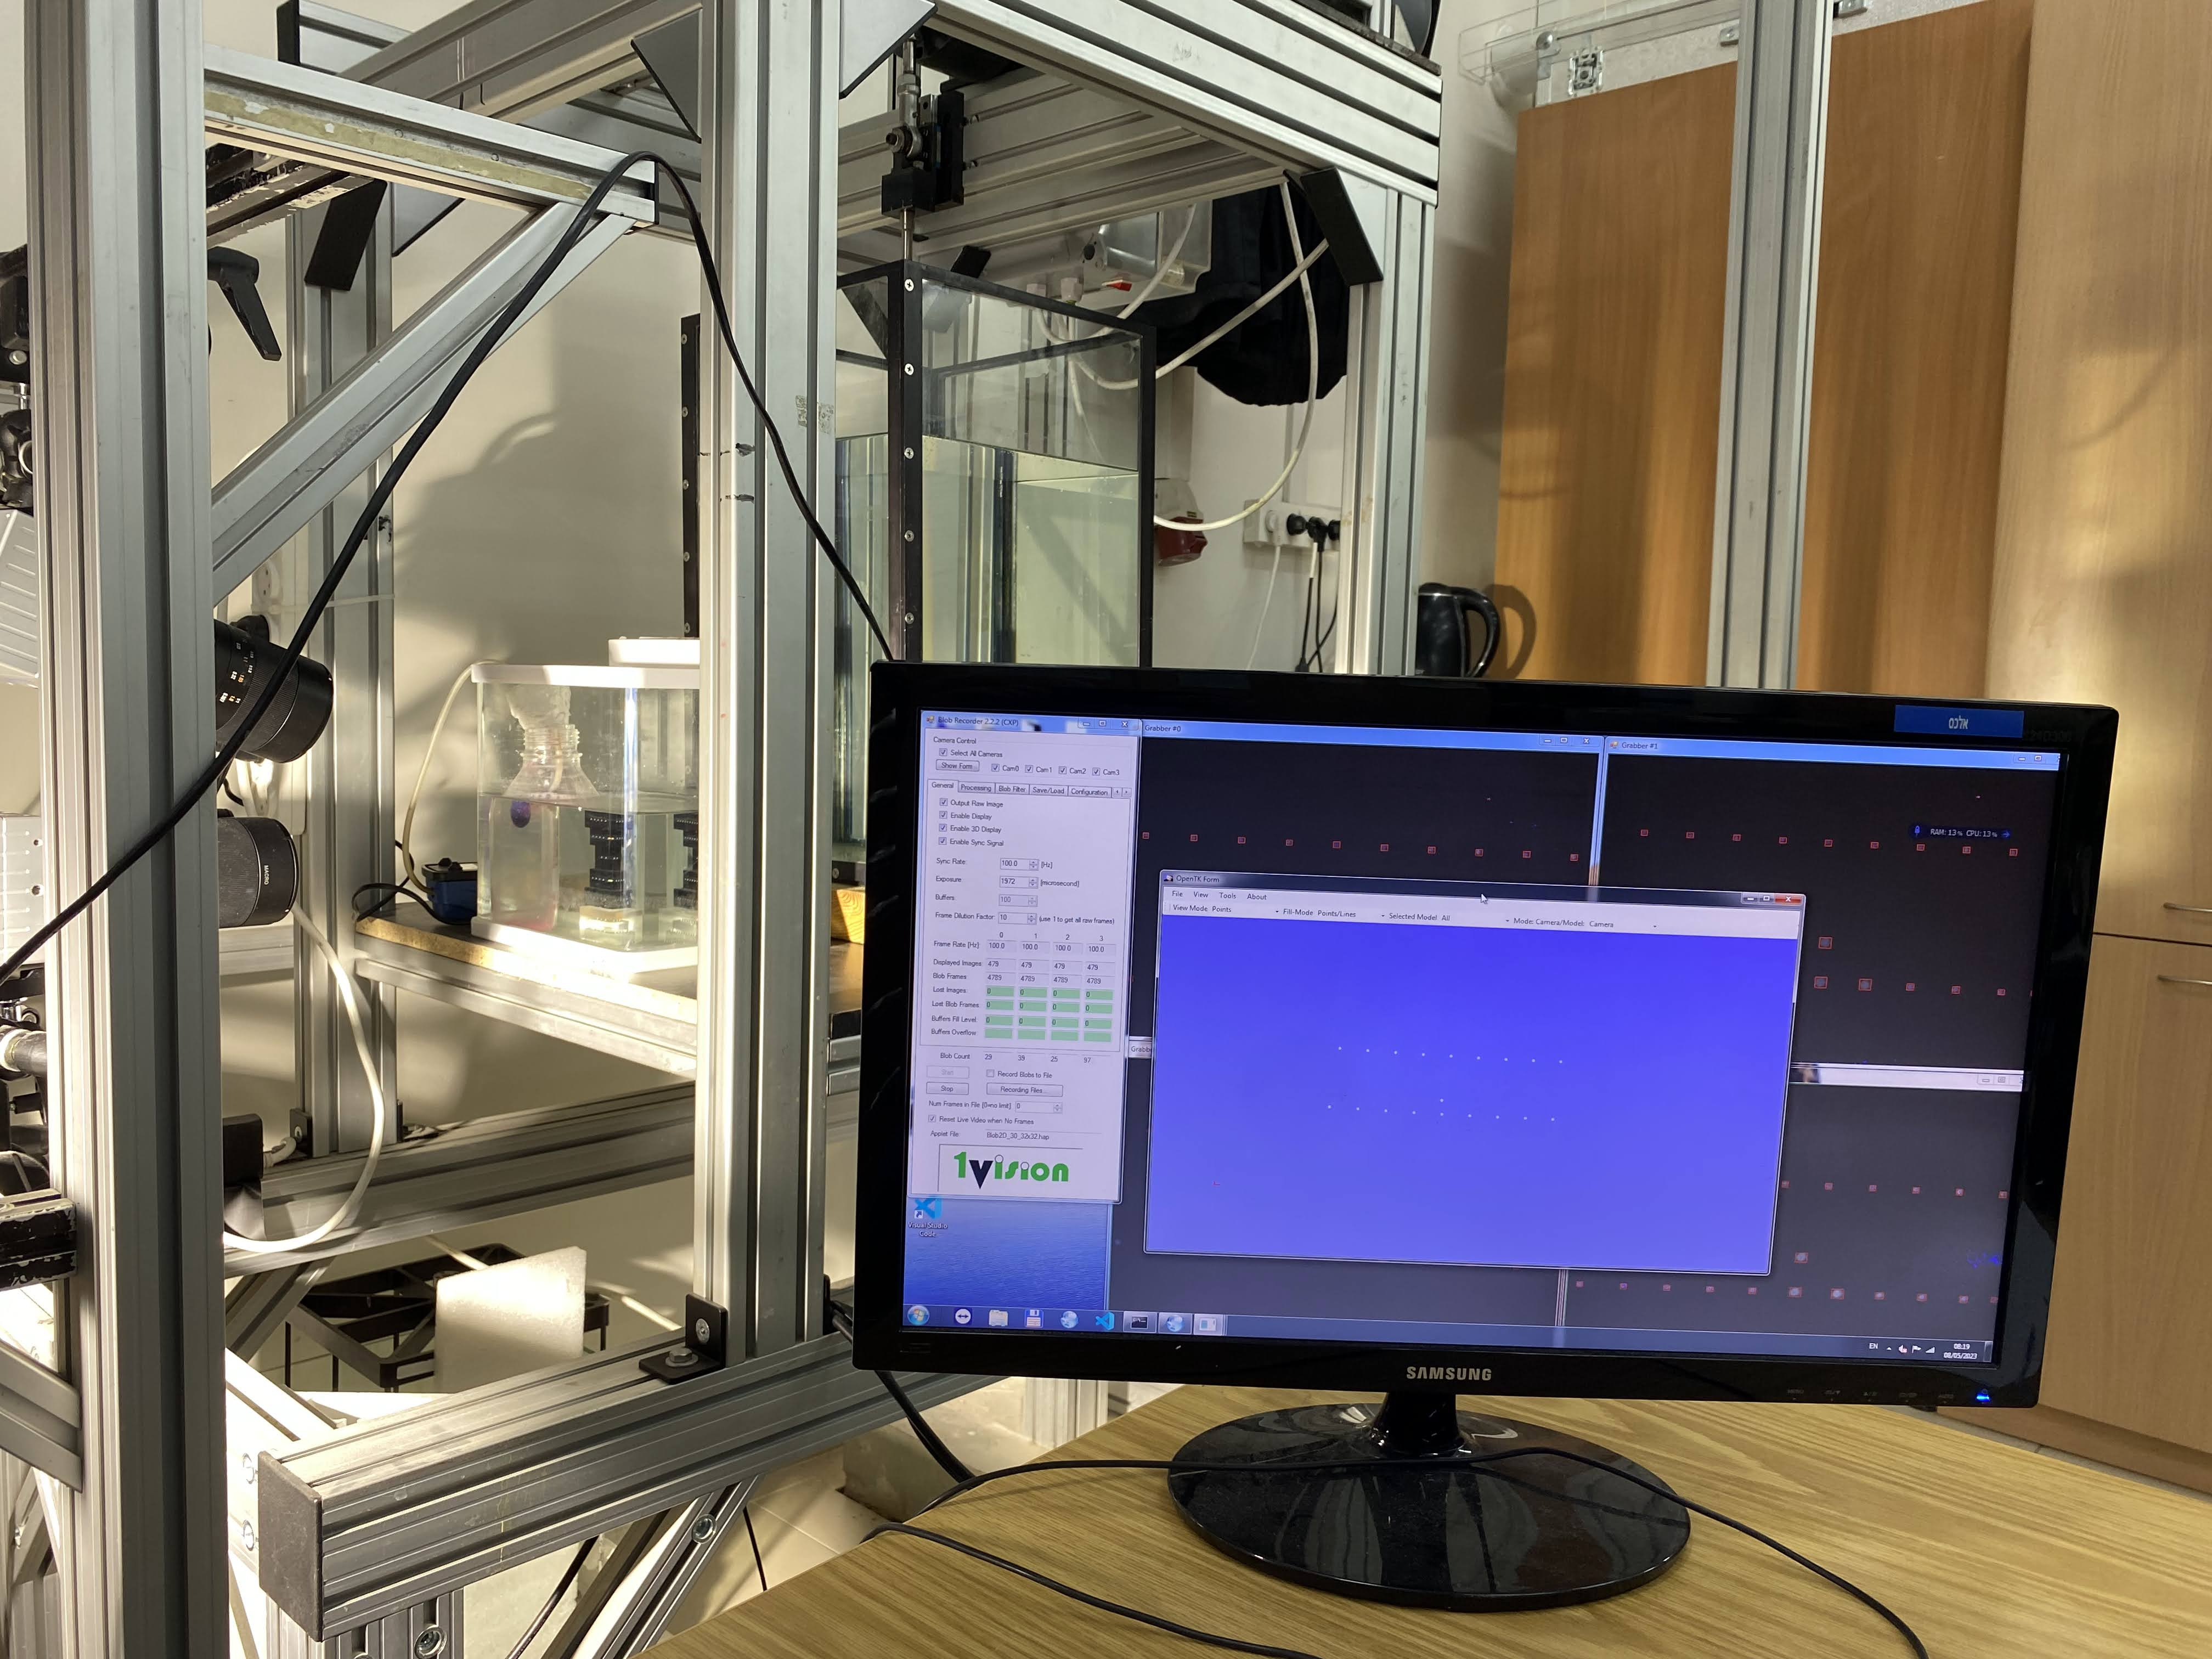
\includegraphics[width=\textwidth]{fig/real_time_3dptv_snapshot.jpg}}{video/real_time_3dptv.mp4}    
\end{frame}


\end{document}














